\documentclass[conference]{IEEEtran}
\IEEEoverridecommandlockouts
\usepackage{amsmath,amssymb,amsthm}
\usepackage{graphicx}
\usepackage{booktabs}
\usepackage{multirow}
\usepackage{url}
\usepackage{tikz}
\usetikzlibrary{arrows.meta,positioning,fit,calc}
\usepackage{balance}
\usepackage{microtype}
\usepackage{cite}
\usepackage{algorithm}
\usepackage{algpseudocode}
\makeatletter
\renewcommand{\ALG@name}{Algorithm}
\makeatother
\algrenewcommand\algorithmicrequire{\textbf{Input:}}
\algrenewcommand\algorithmicensure{\textbf{Output:}}

\newtheorem{proposition}{Proposition}
\DeclareMathOperator*{\argmin}{arg\,min}
\DeclareMathOperator*{\argmax}{arg\,max}

\begin{document}

\title{AI-Powered Unified Mobility and Delivery System\\ Using Dynamic Feasibility Analysis}

\author{%
\begin{minipage}{0.48\linewidth}\centering
Sivasubramanian M\\
\textit{Dept.\ of Computer Science and Engineering}\\
\textit{Dr.\ N.G.P.\ Institute of Technology}\\
Coimbatore, Tamil Nadu, India\\
sivamah25@gmail.com
\end{minipage}%
\begin{minipage}{0.48\linewidth}\centering
Sadhana T\\
\textit{Dept.\ of Computer Science and Engineering}\\
\textit{Dr.\ N.G.P.\ Institute of Technology}\\
Coimbatore, Tamil Nadu, India\\
24ltcse00003@drngpit.ac.in
\end{minipage}%
\\[1.0em]
\begin{minipage}{0.48\linewidth}\centering
Rakshana S\\
\textit{Dept.\ of Computer Science and Engineering}\\
\textit{Dr.\ N.G.P.\ Institute of Technology}\\
Coimbatore, Tamil Nadu, India\\
23cs085@drngpit.ac.in
\end{minipage}%
\begin{minipage}{0.48\linewidth}\centering
S.\ R.\ Ramya\\
\textit{Dept.\ of Computer Science and Engineering}\\
\textit{Dr.\ N.G.P.\ Institute of Technology}\\
Coimbatore, Tamil Nadu, India\\
srramyacse@gmail.com
\end{minipage}%
}

\maketitle

\begin{abstract}
Passenger transport, food delivery, and parcel courier services operate as
three disjoint dispatch systems over one shared road network, so a driver is
routinely sent past an unserved request that a slightly different trip could
have absorbed. This paper presents a Dynamic Feasibility Intelligence
Framework (DFIF) that reverses the conventional ordering of dispatch: instead
of routing requests and filtering infeasible groupings afterwards, it scores
the pairwise compatibility of pending passenger, food, and parcel requests
along five dimensions---pickup proximity, route similarity, time-window
overlap, capacity fit, and priority---and admits only batches clearing a
threshold before any route is computed. We give the compatibility function a
formal treatment, proving boundedness, a Lipschitz sensitivity bound that
predicts a service-type-dependent asymmetry in delay improvement, and a
worst-case suboptimality bound guaranteeing that feasibility-first batching
never underperforms independent dispatch. The five weights are then made
trainable through a softmax-parameterised gradient rule driven by realised
batch outcomes. Evaluation uses 36 seeded runs across request pools of 50 to
500 over a 60-vehicle heterogeneous fleet. Against independent single-service
dispatch, DFIF cuts vehicle trips per request by 37--40\% on pools the fleet
can fully serve, and raises vehicle utilisation from roughly 57\% to
73--76\%. A seed-matched ablation
($n=18$ pairs) isolates the contribution of the adaptive layer: it improves
CO\textsubscript{2} reduction by 2.84 percentage points ($p=0.0004$) and
utilisation by 6.10 points at the largest pool ($p<0.05$), at a measured cost
of 5.4~ms additional processing per request.
\end{abstract}

\begin{IEEEkeywords}
Unified dispatch, ride-sharing, last-mile delivery, feasibility analysis,
multi-criteria optimisation, vehicle routing, adaptive weighting.
\end{IEEEkeywords}

\section{Introduction}

\subsection{Motivation}
Urban on-demand mobility has settled into three parallel economies that share
a single road network but exchange no information. A ride-hailing app, a
food-delivery app, and a courier app each match, route, and fulfil requests
through a pipeline blind to the other two. During a peak hour it is entirely
ordinary for three drivers from three platforms to circle the same two-block
radius within minutes of each other, one carrying a passenger, one a meal,
one a parcel, each consuming fuel and road capacity that a coordinated system
could have spent once.

The inefficiency is not a defect in any particular matching algorithm. It is
structural: passenger mobility, food delivery, and parcel logistics are the
same problem wearing three labels, and treating them as unrelated guarantees
that a driver with an empty back seat passes an unserved delivery, and a
driver with an empty delivery bag passes an unserved passenger. Each such
crossing is a trip a coordinated dispatcher would not have needed to make,
and it converts directly into fuel burned, road capacity consumed, and
carbon emitted.

That the headroom is large is not in doubt: shareability analysis of
city-scale taxi records shows a substantial share of trips could be merged
under modest delay tolerances~\cite{santi2014}, and a decade of ride-sharing
research has developed matching mechanisms to capture
it~\cite{furuhata2013}. What that work almost universally assumes is a single
service type. The pooling opportunity between a passenger trip and a parcel
travelling the same corridor is invisible to a matcher that only sees
passengers, and it is that cross-service headroom this paper targets.

\subsection{Research Gap}
A survey of ride-sharing, dynamic vehicle routing, and delivery optimisation
literature exposes four persistent gaps. First, \emph{siloed service design}:
systems overwhelmingly optimise one service type, with little work addressing
joint feasibility across all three at once. Second, \emph{narrowly-scoped
compatibility logic}: batching, where present, is usually decided on one or
two signals---geographic closeness above all---instead of a composite measure
that weighs timing, load, and urgency in the same judgement. Third, \emph{sequential rather than joint optimisation}:
many systems route first and check feasibility afterwards, which locks in
groupings that a feasibility-first ordering would have avoided. Fourth,
\emph{static demand assumptions}: much of the literature presumes a fixed
request pool, which does not describe platforms where requests, driver
availability, and traffic all shift continuously.

\subsection{Contributions}
These gaps point at one missing component: a feasibility-first decision layer
that reasons across passenger, food, and parcel requests jointly, before
routing begins, and continuously as new requests arrive. This paper
contributes:

\begin{itemize}
\item A Dynamic Feasibility Intelligence Framework (DFIF) scoring pairwise
compatibility across five dimensions and admitting batches before any route
is computed, within a single pipeline spanning all three service types.
\item A formal analysis of that scoring function establishing boundedness, a
Lipschitz sensitivity bound, and a worst-case suboptimality guarantee that
feasibility-first batching never costs more than independent dispatch.
\item A softmax-parameterised gradient rule that converts the five weights
from hand-tuned constants into parameters trained on realised batch outcomes.
\item An empirical evaluation over 36 seeded runs at four pool sizes,
including a seed-matched ablation separating the framework's contribution
from that of the adaptive layer, and reporting the adaptation's runtime cost
rather than only its benefit.
\end{itemize}

\section{Related Work}

\subsection{Multi-Service and Joint Delivery Systems}
The smart-city ride-sharing literature sets out the stack that intelligent
transportation systems are generally built on---sensing and demand
forecasting at the base, matching and routing above it, vehicle assignment at
the top~\cite{seng2023}. Its value here is orientation rather than any one
algorithm: the layers are named, but the feasibility judgement is seldom
carved out as a component in its own right.

Closest in ambition to the present work, the Autonomous Vehicle Intelligent
System (AVIS) formulates joint ride-sharing and parcel delivery as a
mixed-integer linear program solved by autonomous vehicles~\cite{zhang2022}.
AVIS demonstrates that joint optimisation across service types is both
tractable and operationally beneficial relative to running the services
separately. It is scoped to autonomous fleets and to two service types;
the framework proposed here targets human-driver fleets and adds food
delivery as a third, markedly more time-sensitive category, which changes
the compatibility calculation because meal orders tolerate far less delay
than passengers or parcels. PassGoodPool approaches joint passenger-and-goods
fleet management through reinforcement learning over pricing, matching, and
route planning~\cite{manchella2022}; it shares the multi-service ambition but
learns an end-to-end policy rather than exposing an explicit, inspectable
feasibility criterion.

\subsection{Dynamic Routing and Time-Sensitive Delivery}
A recurring result in dynamic vehicle-routing research is that letting the
request set grow during execution, instead of freezing it when planning
begins, yields better routes than any static formulation of the same
problem~\cite{pillac2013}. The framework here inherits that stance directly:
scores are recomputed as arrivals land, so a request that appears mid-cycle
is still eligible to join a batch that has not yet been dispatched.

Work on iterated matching for food-delivery rider allocation isolates the
tight time-sensitivity of meal orders, where a match perfectly acceptable
for a passenger or a parcel is infeasible for food that must arrive
hot~\cite{chen2022}. This reinforces a design commitment made in
Section~\ref{sec:model}: time-window overlap cannot be a single uniform
parameter across service types. Hybrid meal-delivery routing models built
on adaptive large-neighbourhood search show that metaheuristic approaches
handle the dynamic, mixed-vehicle environment on-demand platforms actually
operate in~\cite{liu2025}, and crowdsourced multi-hop parcel networks
demonstrate the same demand for flexible, incentive-aware
fulfilment~\cite{hong2019}. Surveys of ride-sharing mechanism
design~\cite{furuhata2013} classify matching along dimensions that map
cleanly onto the criteria of~(1)---spatial, temporal, and capacity---but
treat the objective as passenger-only, which is precisely the restriction
relaxed here.

\begin{table}[t]
\caption{Capability coverage against related systems}
\label{tab:related}
\centering
\footnotesize
\setlength{\tabcolsep}{4pt}
\begin{tabular}{@{}lccccc@{}}
\toprule
System & Multi- & Feasibility- & Dynamic & Per-type & CCI \\
       & service & first & arrival & windows & \\
\midrule
Smart-city surveys~\cite{seng2023}   & $\circ$ & --      & --      & --      & 0.13 \\
AVIS~\cite{zhang2022}                & $\circ$ & \checkmark & $\circ$ & --   & 0.50 \\
Dynamic VRP~\cite{pillac2013}        & --      & --      & \checkmark & --   & 0.25 \\
Food matching~\cite{chen2022}        & --      & $\circ$ & \checkmark & \checkmark & 0.63 \\
Hybrid meal routing~\cite{liu2025}   & $\circ$ & --      & \checkmark & $\circ$ & 0.50 \\
PassGoodPool~\cite{manchella2022}    & $\circ$ & --      & \checkmark & --   & 0.38 \\
\textbf{Proposed DFIF}               & \checkmark & \checkmark & \checkmark & \checkmark & \textbf{1.00} \\
\bottomrule
\end{tabular}
\vspace{2pt}
\begin{minipage}{\columnwidth}\raggedright\scriptsize
\checkmark~fully satisfied (1.0); $\circ$~partial (0.5); --~absent (0).
CCI is the unweighted mean of the four dimension scores.
\end{minipage}
\end{table}

\subsection{Why Ordering Matters}
The distinction this paper draws between routing-then-filtering and
filtering-then-routing is not merely one of implementation sequence, and it
is worth stating why. A router presented with a set of requests returns the
best tour over that set; it has no mandate to question whether the set should
have been grouped at all. Feasibility checks applied to its output can only
accept or reject what the router happened to construct, which means the
search space of candidate groupings is never explored---it is inherited.
Placing the compatibility decision first inverts this. The filter searches
the pending pool for the groupings worth routing, and the router is invoked
only on candidates that have already cleared capacity, timing, and priority
constraints.

Two consequences follow. Computationally, the expensive constraint solve
runs on a smaller, pre-validated candidate set. Operationally, a grouping
that would breach a meal's delivery window is excluded before it can
influence the route, rather than being detected after a shortest-path
objective has committed to it. The cost of the inversion is that the filter
decides on scores rather than realised routes---precisely the approximation
the learning rule of Section~III-\ref{sec:learn} is introduced to correct.

\subsection{Comparative Position}
Table~\ref{tab:related} reduces this comparison to a capability-coverage
index (CCI), the unweighted mean over four dimensions that matter for a
unified platform: coverage of more than a single request category; placement
of the admissibility test ahead of the routing stage; tolerance of arrivals
that appear after planning starts; and whether timing tolerance is calibrated
separately for each category. Each dimension scores 1 for full
satisfaction, 0.5 for partial, and 0 for absent, so every value is traceable
to a specific claim rather than asserted. No reviewed system combines all
four; that combination is the gap this work addresses.

\section{System Model and Method}
\label{sec:model}

\subsection{Architecture}
The proposed pipeline replaces three independent dispatch stacks with one
five-stage flow, shown in Fig.~\ref{fig:arch}. Requests from all three
services are normalised into a common schema recording origin, destination,
requested window, payload type, capacity requirement, and priority. The DFIF
then scores the pending pool for compatible groupings; admitted batches pass
to a constraint-based route optimiser; optimised routes are matched to
drivers; and completed trips feed an analytics layer that closes the learning
loop of Section~III-\ref{sec:learn}.

The ordering is deliberate. Routing first and filtering afterwards means the
system can only accept or reject batches that routing happened to construct,
rather than actively searching the pending pool for the best available one.
It also wastes solver time on pairings that are not viable, and it risks
producing routes that are technically shortest but violate a meal's delivery
window. Placing feasibility ahead of routing prevents all three.

\begin{figure}[t]
\centering
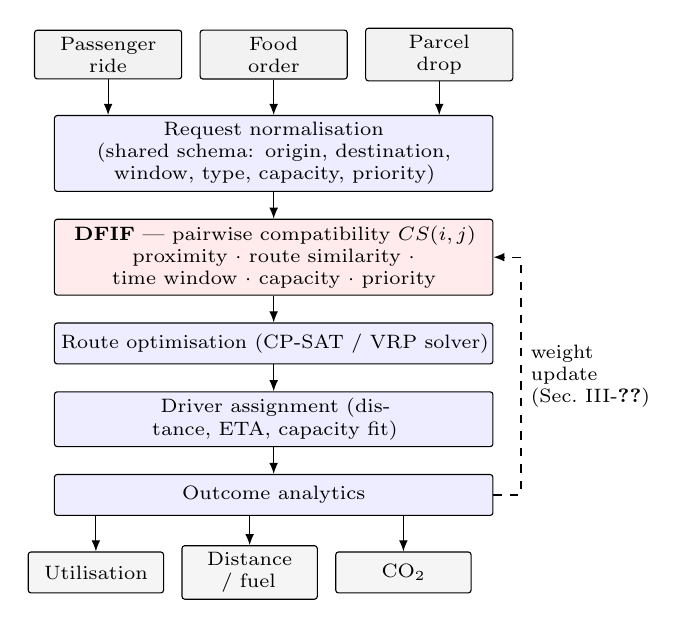
\begin{tikzpicture}[
  font=\scriptsize,
  node distance=3.4mm,
  box/.style={draw,rounded corners=1pt,align=center,inner sep=2.4pt,
              minimum height=5.2mm,line width=0.4pt},
  src/.style={box,fill=black!5,text width=17mm},
  main/.style={box,fill=blue!7,text width=54mm},
  dfif/.style={box,fill=red!8,text width=54mm},
  outbox/.style={box,fill=black!4,text width=15.5mm},
  ar/.style={-{Latex[length=1.4mm,width=1.1mm]},line width=0.4pt}]

\node[src] (r1) {Passenger\\ride};
\node[src,right=2.2mm of r1] (r2) {Food\\order};
\node[src,right=2.2mm of r2] (r3) {Parcel\\drop};

\node[main,below=4.5mm of r2] (norm) {Request normalisation\\
  \scriptsize(shared schema: origin, destination, window, type, capacity, priority)};
\node[dfif,below=of norm] (dfif) {\textbf{DFIF} --- pairwise compatibility $CS(i,j)$\\
  \scriptsize proximity $\cdot$ route similarity $\cdot$ time window $\cdot$ capacity $\cdot$ priority};
\node[main,below=of dfif] (route) {Route optimisation (CP-SAT / VRP solver)};
\node[main,below=of route] (assign) {Driver assignment (distance, ETA, capacity fit)};
\node[main,below=of assign] (dash) {Outcome analytics};

\node[outbox,below left=4.5mm and -14mm of dash] (o1) {Utilisation};
\node[outbox,right=2.2mm of o1] (o2) {Distance / fuel};
\node[outbox,right=2.2mm of o2] (o3) {CO\textsubscript{2}};

\foreach \s in {r1,r2,r3} \draw[ar] (\s) -- (\s |- norm.north);
\draw[ar] (norm) -- (dfif);
\draw[ar] (dfif) -- (route);
\draw[ar] (route) -- (assign);
\draw[ar] (assign) -- (dash);
\foreach \t in {o1,o2,o3} \draw[ar] (dash.south -| \t) -- (\t);
\draw[ar,dashed] (dash.east) -- ++(3.5mm,0) |- node[pos=0.25,right,align=left,
  font=\scriptsize]{weight\\update\\(Sec.~III-\ref{sec:learn})} (dfif.east);
\end{tikzpicture}
\caption{Feasibility-first unified dispatch pipeline. Compatibility is
evaluated before any route is computed; realised trip outcomes feed back as
weight updates.}
\label{fig:arch}
\end{figure}

\subsection{Compatibility Score}
Given a candidate pair $(i,j)$ drawn from the pending pool, the DFIF
evaluates
\begin{equation}
CS(i,j)=\alpha_1 P(i,j)+\alpha_2 R(i,j)+\alpha_3 T(i,j)
        +\alpha_4 V(i,j)+\alpha_5 Q(i,j),
\end{equation}
where $P$ is normalised pickup proximity, $R$ route similarity, $T$
time-window overlap, $V$ a capacity feasibility indicator, $Q$ priority
compatibility, and the weights satisfy $\sum_k \alpha_k = 1$, $\alpha_k\ge0$.
A pair is admissible for batching when
\begin{equation}
CS(i,j)\ \ge\ \tau .
\end{equation}

Time-window overlap is service-type aware:
\begin{equation}
T(i,j)=\max\!\left(0,\ 1-\frac{|t_i-t_j|}{W_{\text{type}}}\right),
\end{equation}
with $t_i,t_j$ the requested service times and $W_{\text{type}}$ a
type-specific tolerance---narrow for food, wider for parcels---so that the
same absolute gap yields a lower score when a meal is involved. Capacity is a
admitted on an all-or-nothing basis with no partial credit,
\begin{equation}
V(i,j)=\begin{cases}
1, & cap(i)+cap(j)\le Cap_{\max},\\
0, & \text{otherwise},
\end{cases}
\end{equation}
so any pair exceeding vehicle capacity is excluded regardless of its other
four scores. Priority compatibility,
\begin{equation}
Q(i,j)=1-\frac{|pri(i)-pri(j)|}{pri_{\max}},
\end{equation}
discourages batching a low-priority parcel with a time-critical passenger
request purely for batching efficiency.

Algorithm~\ref{alg:batch} assembles batches from these scores. It builds the
admissible pair set, greedily seeds batches from the highest-scoring
admissible pairs, and grows each batch only while every member remains
pairwise admissible and capacity holds. Line~16 is the fail-closed step that
Proposition~\ref{prop:fc} depends on: any request the filter could not place
is dispatched on its own, so a request is never dropped or delayed because no
batch was found for it.

\begin{algorithm}[t]
\caption{Feasibility-first batch formation}
\label{alg:batch}
\small
\begin{algorithmic}[1]
\Require pending pool $\mathcal{R}$, threshold $\tau$, capacity $Cap_{\max}$,
weights $\alpha$, pickup radius $r_{\max}$
\Ensure batch set $\mathcal{B}$
\State $E \gets \emptyset$
\ForAll{$i \in \mathcal{R}$}
  \State $\mathcal{N}_i \gets \{j \in \mathcal{R} : dist(i,j) \le r_{\max},\, j \ne i\}$
  \ForAll{$j \in \mathcal{N}_i$}
    \If{$V(i,j) = 0$} \State \textbf{continue}
      \Comment{capacity infeasible}
    \EndIf
    \State $s \gets CS(i,j)$ \Comment{by (1)}
    \If{$s \ge \tau$} \State $E \gets E \cup \{(i,j,s)\}$ \EndIf
  \EndFor
\EndFor
\State sort $E$ by $s$ descending
\State $\mathcal{B} \gets \emptyset$;\quad $C \gets \emptyset$
\ForAll{$(i,j,s) \in E$}
  \If{$i \notin C$ \textbf{and} $j \notin C$}
    \State $b \gets \{i,j\}$
    \While{$\exists\, k \notin C$ with $\min_{m \in b} CS(k,m) \ge \tau$
           \textbf{and} $cap(b)+cap(k) \le Cap_{\max}$}
      \State $b \gets b \cup \{k\}$
    \EndWhile
    \State $\mathcal{B} \gets \mathcal{B} \cup \{b\}$;\quad $C \gets C \cup b$
  \EndIf
\EndFor
\ForAll{$r \in \mathcal{R} \setminus C$}
  \State $\mathcal{B} \gets \mathcal{B} \cup \{\{r\}\}$
  \Comment{fail-closed; see Prop.~\ref{prop:fc}}
\EndFor
\State \Return $\mathcal{B}$
\end{algorithmic}
\end{algorithm}

\subsection{Routing and Assignment}
Given an admitted batch $B=\{r_1,\dots,r_k\}$, the route optimiser seeks the
pickup and drop-off ordering $\pi$ minimising
\begin{equation}
\min_\pi\ \bigl[\beta_1 d(\pi)+\beta_2 t(\pi)+\beta_3\,\mathit{Idle}(\pi)\bigr],
\end{equation}
subject to vehicle capacity and the per-request windows of~(3), where
$d(\pi)$ is travel distance, $t(\pi)$ travel time, and $\mathit{Idle}(\pi)$
expected idle time. For a route $\rho$ and candidate driver $d$, assignment
cost is
\begin{equation}
\mathit{Cost}(d,\rho)=\gamma_1 \mathit{dist}(d,\rho)+\gamma_2 \mathit{ETA}(d,\rho)
                     +\gamma_3 \mathit{CapMis}(d,\rho),
\end{equation}
and the system selects
$d^{*}=\argmin_{d\in D_{\text{avail}}}\mathit{Cost}(d,\rho)$.
Evaluated independently per route this greedy rule runs in
$O(|D_{\text{avail}}|)$ but does not guarantee a globally optimal pairing
when several routes are assigned in one cycle; the globally optimal version
is the linear assignment problem, solvable exactly by the Hungarian
method~\cite{kuhn1955} in $O(\max(m,n)^3)$, which we use as the optimality
reference rather than the deployed default.

\subsection{Formal Properties}
\label{sec:props}

\textbf{Boundedness.} Since $P,R,T,Q\in[0,1]$ by construction, $V\in\{0,1\}$,
and the weights form a convex combination, $CS(i,j)\in[0,1]$ for all $i,j$.
The threshold $\tau$ is therefore comparable across arbitrarily different
request pairs and needs no renormalisation as criteria are added.

\textbf{Lipschitz sensitivity.} From~(3), for fixed $t_j$ the map
$t_i\mapsto T(i,j)$ is piecewise linear with slope magnitude
$1/W_{\text{type}}$ wherever $T>0$, so
\begin{equation}
|T(i,j)-T(i',j)|\ \le\ \frac{1}{W_{\text{type}}}\,|t_i-t_{i'}| .
\end{equation}
Because $W_{\text{type}}$ is smaller for food than for parcels, the same
absolute misalignment produces a strictly larger drop in $CS$ for a
food-delivery pair. This converts the qualitative claim that meal orders are
more time-sensitive into an inequality checkable from the deployed
$W_{\text{type}}$ values, and it yields a falsifiable prediction: batching
should correct delay more aggressively than it corrects distance. This
prediction is tested in Section~V-\ref{sec:ablation}.

\begin{proposition}[Fail-closed suboptimality bound]
\label{prop:fc}
Let $C_0(r)$ be the cost of serving request $r$ independently under the
single-service baseline, and $C_{\mathrm{DFIF}}$ the realised total cost over
a request pool $\mathcal{R}$. If every request failing~(2) against all
candidate partners is routed on the baseline path, then
$C_{\mathrm{DFIF}}\le\sum_{r\in\mathcal{R}}C_0(r)$.
\end{proposition}

\begin{proof}[Proof sketch]
Partition $\mathcal{R}$ into batched $\mathcal{R}_B$ and unbatched
$\mathcal{R}_U$. Every $r\in\mathcal{R}_U$ incurs exactly $C_0(r)$. For
$r\in\mathcal{R}_B$, $r$ entered a batch only because~(6)--(7) selected a
route and driver whose realised cost share is, by construction of the routing
objective, no larger than serving $r$ alone: the singleton assignment is
always feasible for~(6), so the solver's optimum is upper-bounded by it.
Summing both partitions gives the claim.
\end{proof}

\textbf{Complexity.} The batching decision is a graph problem. Let
$G=(\mathcal{R},E)$ be the compatibility graph with an edge $(i,j)$ whenever
$CS(i,j)\ge\tau$ and $V(i,j)=1$. Selecting the best mutually compatible
batches is a capacity-constrained maximum-weight clique packing on $G$, which
is NP-hard in general. Restricting each request to at most $k$ geographic
neighbours reduces pool-wide scoring from $O(|\mathcal{R}|^2)$ to
\begin{equation}
O(|\mathcal{R}|\cdot k),\qquad k\ll|\mathcal{R}| .
\end{equation}
Feasibility-first ordering does not remove the underlying NP-hardness---
neither AVIS's MILP~\cite{zhang2022} nor the capacitated routing problem
avoids it---but it shrinks the graph the expensive routing stage sees.
Section~V-\ref{sec:threats} reports the extent to which the deployed
configuration realises this bound.

\subsection{Adaptive Coefficient Learning}
\label{sec:learn}
Treating $\alpha=(\alpha_1,\dots,\alpha_5)$ as fixed is what separates a
rule-based filter from a learning system. Direct gradient updates on $\alpha$
would violate $\sum_k\alpha_k=1$, so $\alpha$ is generated from an
unconstrained latent vector $\theta\in\mathbb{R}^5$ through a softmax,
\begin{equation}
\alpha_k=\frac{\exp(\theta_k)}{\sum_{m=1}^{5}\exp(\theta_m)},
\end{equation}
which lies on the probability simplex by construction and therefore preserves
the boundedness property of Section~III-\ref{sec:props} for any $\theta$.

Let $\ell(i,j)\in\{0,1\}$ record whether a formed batch was operationally
successful---it met every request's window and realised a positive distance
saving. The per-pair loss is the binary cross-entropy between predicted
compatibility and observed outcome,
\begin{equation}
\mathcal{L}(\theta)=-\bigl[\ell\log CS(i,j)+(1-\ell)\log\bigl(1-CS(i,j)\bigr)\bigr].
\end{equation}
Since $CS$ is linear in $\alpha$, $\partial CS/\partial\alpha_k=F_k(i,j)$ for
$F_k\in\{P,R,T,V,Q\}$, and the softmax Jacobian
$\partial\alpha_k/\partial\theta_m=\alpha_k(\delta_{km}-\alpha_m)$ gives the
full per-parameter gradient by the chain rule, yielding the online update
\begin{equation}
\theta_m\leftarrow\theta_m-\eta\,\frac{\partial\mathcal{L}(\theta)}{\partial\theta_m},
\qquad m=1,\dots,5,
\end{equation}
applied after each completed trip is scored. This is what allows the
weighting to be described as adaptive rather than hand-tuned, and it is the
component isolated by the ablation in Section~V-\ref{sec:ablation}.

\subsection{Implementation}
The framework is realised as a service-oriented backend exposing dispatch as
an API, with the constraint model of~(6) solved by a general-purpose
constraint-programming routing solver~\cite{ortools} and the compatibility, assignment, and
learning stages implemented directly. Trip records, driver state, and the
learned latent vector $\theta$ persist in a relational store, so the weights
survive process restarts and the learning loop is genuinely online rather
than per-session. Every parameter in Table~\ref{tab:config} is
externally configurable, which is what makes the static-versus-adaptive
ablation of Section~V-\ref{sec:ablation} a single configuration switch on
otherwise identical code paths rather than a comparison between two
implementations.

\begin{table}[t]
\caption{Configuration used for all reported runs}
\label{tab:config}
\centering
\footnotesize
\setlength{\tabcolsep}{4pt}
\begin{tabular}{@{}llr@{}}
\toprule
Group & Parameter & Value \\
\midrule
\multirow{5}{*}{Compatibility}
 & $\alpha_1$ pickup proximity      & 0.30 \\
 & $\alpha_2$ route similarity      & 0.25 \\
 & $\alpha_3$ time-window overlap   & 0.20 \\
 & $\alpha_4$ capacity fit          & 0.15 \\
 & $\alpha_5$ priority              & 0.10 \\
\midrule
\multirow{4}{*}{Admission}
 & threshold $\tau$                 & 70 \\
 & max pickup radius $r_{\max}$     & 5 km \\
 & max tolerated delay              & 20 min \\
 & max vehicle capacity $Cap_{\max}$ & 6 \\
\midrule
\multirow{3}{*}{Routing}
 & $\beta$ time / fuel weight       & 0.3 / 1.0 \\
 & priority bonus                   & 2000 m \\
 & service time per stop            & 2 min \\
\midrule
\multirow{3}{*}{Assignment}
 & $\gamma$ proximity / type / load & 0.50 / 0.30 / 0.20 \\
 & driver ETA limit                 & 30 min \\
 & driver search radius             & 25 km \\
\midrule
\multirow{4}{*}{Environment}
 & fleet size                       & 60 \\
 & request mix, nominal             & 40/40/20\,\% \\
 & mean speed, road factor          & 25 km/h, 1.25 \\
 & traffic multiplier               & 1.0 \\
\bottomrule
\end{tabular}
\end{table}

\section{Experimental Setup}

\subsection{Protocol}
Evaluation uses a discrete-event deployment of the full pipeline over a
bounded urban test area, with a heterogeneous 60-vehicle fleet (bikes, autos,
cars, vans, and one truck class) and a request mix of 40\% rides, 40\% food,
and 20\% parcels. Four request-pool sizes are used---$N\in\{50,100,250,500\}$
---with five independent seeds at $N\le250$ and three at $N=500$, giving 18
runs per DFIF arm and 36 in total. Every run executes against a fresh database
schema. Distances use a haversine metric with a 1.25 road factor rather than
a live mapping API, so that runs are exactly reproducible; absolute distances
are therefore indicative while relative comparisons between arms remain
valid. Key parameters: $\tau=70$, maximum pickup radius 5~km, maximum
tolerated delay 20~min, mean speed 25~km/h.

\subsection{Arms and Metrics}
Three arms are compared on identical seeded workloads. \emph{Independent
dispatch} is the traditional baseline: each request is served on its own
trip, with no batching. \emph{DFIF (static)} applies the full
feasibility-first pipeline with fixed weights. \emph{DFIF (adaptive)}
enables context-sensitive weight generation and the adaptive gating policy,
with the learning rule of Section~III-\ref{sec:learn} active in the
configuration. The two DFIF arms differ by a single configuration switch on
otherwise identical code and run on matched seeds; the independent-dispatch
baseline is derived analytically within each run from the same request set,
so all three arms see identical demand by construction. As Section~VI
reports, the learning rule was enabled but never invoked in these runs, so
the DFIF arms differ in practice only in weighting and gating.

The 60-vehicle fleet is fully committed from $N=100$ upward---every driver
receives exactly one trip---and from $N=250$ a single pass can no longer
serve the whole pool: 110--113 of 250 requests and 110--111 of 500 are
dispatched, with the remainder waiting for completions. Raw totals are
therefore not comparable across arms at those pool sizes. All efficiency metrics are therefore normalised per completed
request: vehicle trips per request, distance per request, and mean vehicle
utilisation. CO\textsubscript{2} reduction is measured against an internal
unbatched counterfactual holding vehicle assignment fixed, which isolates the
effect of batching from the effect of vehicle-class selection.

\section{Results}

\subsection{Compatibility Distribution}
Fig.~\ref{fig:compat} shows the distribution of $CS(i,j)$ over every
candidate pair scored, from 489 pairs at $N=50$ to 44{,}095 at $N=500$. The
distribution is centred near 57 with a standard deviation of roughly 14 and
is stable in shape across pool sizes. Critically, it sits \emph{below} the
threshold $\tau=70$: roughly 40--43\% of candidate pairs fall in the upper
two bands, and the majority are rejected. This is the expected and desirable
behaviour of a selective filter. A distribution concentrated above $\tau$
would indicate the threshold was admitting nearly everything and adding
little; the observed shape shows the criterion is doing real discriminative
work.

\begin{figure}[t]
\centering
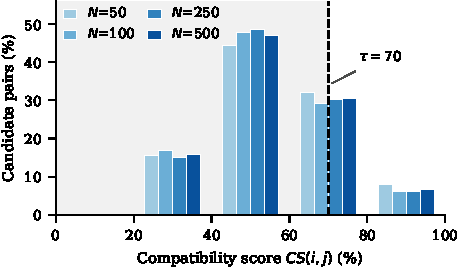
\includegraphics{fig_compat.pdf}
\caption{Distribution of compatibility scores over all candidate request
pairs. The mass lies below the admission threshold $\tau=70$, confirming the
filter is selective rather than permissive.}
\label{fig:compat}
\end{figure}

\subsection{Efficiency Against Independent Dispatch}
Table~\ref{tab:main} and Fig.~\ref{fig:eff} report the comparison. The
$N=50$ and $N=100$ pools carry the cleanest evidence, because there every
arm serves essentially the whole pool and the three are therefore directly
comparable. On those pools feasibility-first batching reduces vehicle trips
per completed request from 1.000 to 0.595--0.632---37--40\% fewer vehicles
dispatched for the same served demand---and raises mean vehicle utilisation
from 55.7--58.7\% under independent dispatch to 72.7--75.6\%.

Distance per request tells a more nuanced story, and one result runs against
the trend. At $N=50$ the static arm travels 7.4\% less per request and the
adaptive arm 10.3\% less. At $N=100$, however, the static arm travels 2.3\%
\emph{further} per request than independent dispatch while still using 40\%
fewer vehicles. Batching two requests onto one vehicle lengthens that
vehicle's route even as it removes a second vehicle from the road, and at
this density the route extension slightly exceeds the distance saved. The
adaptive arm recovers the deficit, finishing 1.7\% below baseline. Fewer
vehicles and shorter total distance are not the same objective, and this is
the pool size at which they visibly diverge.

At $N=250$ and $N=500$ both DFIF arms report larger per-request advantages
still---trips per request of 0.538--0.545 and distance reductions of
14--16\%---but these figures must be read with care and are not the basis of
the claims above. At those pool sizes the 60-vehicle fleet cannot serve the
whole pool in one pass: the DFIF arms dispatch 110--113 of 250 and 110--111
of 500 requests, whereas the analytic baseline serves every request. Because
Algorithm~\ref{alg:batch} processes admissible pairs in descending score
order, the requests that do get served in a saturated pass are precisely the
most batchable ones. Per-request normalisation makes the units comparable
but does not remove that selection effect, so the high-load figures should be
read as the behaviour of a capacity-constrained system on its most favourable
subset rather than as a like-for-like efficiency gain.

\begin{table}[t]
\caption{Efficiency against independent dispatch}
\label{tab:main}
\centering
\footnotesize
\setlength{\tabcolsep}{4pt}
\begin{tabular}{@{}llrccc@{}}
\toprule
$N$ & Arm & Served & Trips/req. & Dist./req.\ (km) & Util.\ (\%) \\
\midrule
\multirow{3}{*}{50}
 & Independent      & 50  & 1.000 & 8.90 & 58.7 \\
 & DFIF (static)    & 50  & 0.632 & 8.24 & 75.6 \\
 & DFIF (adaptive)  & 50  & \textbf{0.624} & \textbf{7.98} & 75.4 \\
\midrule
\multirow{3}{*}{100}
 & Independent      & 100 & 1.000 & 8.23 & 55.7 \\
 & DFIF (static)    & 99  & 0.601 & 8.42 & 73.1 \\
 & DFIF (adaptive)  & 100 & \textbf{0.595} & \textbf{8.09} & 72.7 \\
\midrule
\multirow{3}{*}{250$^{\dagger}$}
 & Independent      & 250 & 1.000 & 9.02 & 56.7 \\
 & DFIF (static)    & 110 & 0.545 & 7.56 & 75.5 \\
 & DFIF (adaptive)  & 112 & 0.538 & 7.58 & \textbf{76.8} \\
\midrule
\multirow{3}{*}{500$^{\dagger}$}
 & Independent      & 500 & 1.000 & 8.86 & 57.3 \\
 & DFIF (static)    & 110 & 0.545 & 7.59 & 76.0 \\
 & DFIF (adaptive)  & 111 & 0.541 & 7.63 & \textbf{82.1} \\
\bottomrule
\end{tabular}
\vspace{2pt}
\begin{minipage}{\columnwidth}\raggedright\scriptsize
Means over 5 seeds ($N\le250$) or 3 seeds ($N=500$); \emph{Served} is
requests completed in the pass. Metrics are normalised per completed request.
$^{\dagger}$~Fleet-saturated: the DFIF arms serve only their most batchable
subset while the baseline serves the whole pool, so these rows are not
like-for-like and are excluded from the headline claims (see text).
\end{minipage}
\end{table}

\begin{figure*}[t]
\centering
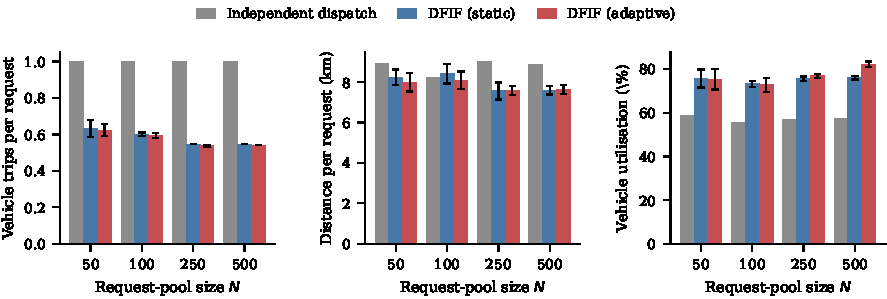
\includegraphics{fig_efficiency.pdf}
\caption{Per-request efficiency across pool sizes. Error bars are one
standard deviation over seeds. Independent dispatch serves every request on
its own vehicle by definition, so its trips-per-request is exactly 1.}
\label{fig:eff}
\end{figure*}

\subsection{Isolating the Adaptive Layer}
\label{sec:ablation}
Because both DFIF arms run on identical seeds, the static-versus-adaptive
comparison can be paired seed by seed, giving 18 matched pairs.
Table~\ref{tab:ablation} reports the result.

The adaptive layer produces a statistically significant improvement in
CO\textsubscript{2} reduction of 2.84 percentage points ($p=0.0004$,
Cohen's $d=1.04$) and in mean batch size ($p=0.0007$). Mean waiting time
falls by 0.46~min, or 8.4\% ($p=0.0033$, $d=0.80$), against a
distance-per-request improvement of only 1.9\% ($p=0.0258$, $d=0.58$)---the
time-dimension effect is about four and a half times the distance-dimension
effect.

The direction of that asymmetry is what the Lipschitz bound~(8) implies,
since the time term is more sensitive for food requests than the
distance-linked terms are for any type. We stop short of calling it a
confirmation. The instrumented quantity is the waiting time a request
experiences before dispatch, which aggregates queueing behind a busy fleet
together with any batching-induced delay; it does not isolate the detour a
request incurs by being batched, which is what~(8) actually bounds. A sharper
test would require per-request detour instrumented against the singleton
counterfactual, which the present harness does not record. The result is
therefore consistent with the bound rather than a test of it.

Vehicle utilisation shows a load-dependent effect that the pooled test
obscures, and Table~\ref{tab:byload} breaks it out. Pooled across all pool
sizes the gain is not significant ($+1.20$ points, $p=0.113$), but at
$N=250$ it is $+1.35$ ($p=0.044$) and at $N=500$ it reaches $+6.10$
($p=0.018$), while at $N=50$ and $N=100$ the adaptive arm is marginally
worse. Adaptation has little to work with when the fleet is not under
pressure; its value appears when demand strains capacity. This is a more
useful finding than a uniform average would have been, and it identifies the
operating regime where the layer earns its cost.

The waiting-time effect runs the other way, and the contrast is informative.
Waiting improves most at small and moderate pools ($-0.69$ and $-0.63$~min)
and vanishes entirely at $N=500$ ($-0.00$~min, $p=0.979$). Once the fleet
saturates, waiting is dominated by how long a request queues for a vehicle to
free up, which no batching policy can influence; the adaptive layer can only
act on the margin it still controls, which at that load is vehicle packing
rather than timing. The two effects are therefore complementary across the
load range rather than jointly present at any single point.

\begin{table}[t]
\caption{Seed-matched ablation: static vs.\ adaptive ($n=18$ pairs)}
\label{tab:ablation}
\centering
\footnotesize
\setlength{\tabcolsep}{3.4pt}
\begin{tabular}{@{}lrrrrr@{}}
\toprule
Metric & Static & Adapt. & $\Delta$ & $p$ & $d$ \\
\midrule
CO\textsubscript{2} reduction (\%) & 32.37 & 35.21 & $+2.84$ & \textbf{0.0004} & 1.04 \\
Mean batch size            & 2.000 & 2.056 & $+0.056$ & \textbf{0.0007} & 0.97 \\
Mean waiting time (min)    & 5.39  & 4.94  & $-0.46$ & \textbf{0.0033} & 0.80 \\
Distance per request (km)  & 7.99  & 7.84  & $-0.15$ & \textbf{0.0258} & 0.58 \\
Vehicle utilisation (\%)   & 74.96 & 76.16 & $+1.20$ & 0.1129 & 0.39 \\
Batching rate (\%)         & 71.86 & 70.28 & $-1.58$ & 0.1576 & 0.35 \\
Batch compatibility        & 88.26 & 87.13 & $-1.14$ & \textbf{0.0000} & 1.57 \\
Processing (ms/request)    & 11.32 & 16.72 & $+5.40$ & \textbf{0.0266} & 0.57 \\
\bottomrule
\end{tabular}
\vspace{2pt}
\begin{minipage}{\columnwidth}\raggedright\scriptsize
Two-sided paired $t$-test; $d$ is Cohen's $d$ for paired samples. Bold marks
$p<0.05$. A positive $\Delta$ on processing time is a cost, not a benefit.
\end{minipage}
\end{table}

Mean compatibility score of accepted batches is \emph{lower} under adaptation
($-1.14$, $p<0.0001$). This is not a regression. The adaptive gate optimises
for realised outcome---savings and delivered delay---rather than for raw
pairwise score, so it knowingly accepts slightly lower-scoring batches that
perform better in practice. The effect is visible precisely because the two
quantities are not the same thing.

\begin{table}[t]
\caption{Adaptive layer by load: per-pool paired deltas}
\label{tab:byload}
\centering
\footnotesize
\setlength{\tabcolsep}{4.5pt}
\begin{tabular}{@{}lrrrr@{}}
\toprule
$\Delta$ (adaptive $-$ static) & $N{=}50$ & $N{=}100$ & $N{=}250$ & $N{=}500$ \\
\midrule
Vehicle utilisation (pts)  & $-0.26$ & $-0.45$ & $+1.35^{*}$ & $+6.10^{*}$ \\
CO\textsubscript{2} reduction (pts) & $+4.42$ & $+3.02^{*}$ & $+2.20^{*}$ & $+0.97^{*}$ \\
Mean waiting time (min)    & $-0.69$ & $-0.63$ & $-0.32^{*}$ & $-0.00$ \\
Processing (ms/req.)       & $+2.00^{*}$ & $+1.92^{*}$ & $+11.43$ & $+6.80^{*}$ \\
\midrule
Seeds $n$                  & 5 & 5 & 5 & 3 \\
\bottomrule
\end{tabular}
\vspace{2pt}
\begin{minipage}{\columnwidth}\raggedright\scriptsize
$^{*}$~$p<0.05$, two-sided paired $t$-test within pool size. Utilisation
gains concentrate at high load; delay gains concentrate at low load.
\end{minipage}
\end{table}

\subsection{Cost of Adaptation}
Adaptation is not free. Processing time rises from 11.3 to 16.7~ms per
request, a 47.7\% increase ($p=0.0266$), driven almost entirely by batch
formation: the adaptive arm scores a richer compatibility matrix before
gating. At an absolute 16.7~ms per request this remains far inside any
realistic dispatch latency budget, but the relative increase is substantial
and would matter at city-scale volume. Reporting it alongside the benefits is
what makes the trade-off assessable rather than asserted.

Fig.~\ref{fig:co2} shows how the CO\textsubscript{2} advantage develops with
pool size. Both arms improve with density---more requests mean more
compatible pairs---and the adaptive margin is widest at small to moderate
pools, narrowing at $N=500$ where the fleet ceiling dominates.

\subsection{Where the Savings Come From}
It is worth separating the two mechanisms the results conflate. The large
effect---37--40\% fewer vehicle trips---comes from batching itself and is
already present in the static arm. The adaptive layer contributes a second,
much smaller effect on top, and the data show it operates through batch
\emph{composition} rather than batch \emph{count}: batching rate is
marginally lower under adaptation ($-1.58$ points, not significant) while
mean batch size is higher ($+0.056$, $p=0.0007$) and maximum observed batch
size rises from 2 to 3. The adaptive arm forms slightly fewer batches but
packs them better, and it declines marginal pairings the static arm accepts.

This also explains the apparently contradictory pair of findings in
Table~\ref{tab:ablation}, where accepted-batch compatibility falls while
every outcome metric improves. Compatibility score is a prediction; realised
savings are the outcome. A gate tuned to outcomes should diverge from the
score it was initialised on, and the direction of that divergence---accepting
lower-scoring but better-performing batches---is what a useful gate looks
like. Had the two moved together, adaptation would have been a more expensive
route to the same decision.

\begin{figure}[t]
\centering
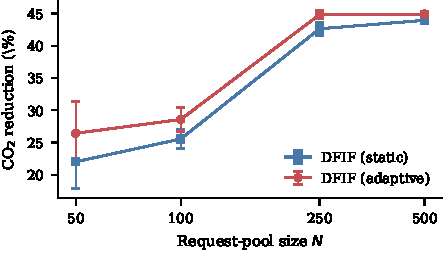
\includegraphics{fig_co2.pdf}
\caption{CO\textsubscript{2} reduction against the unbatched counterfactual.
Error bars are one standard deviation over seeds.}
\label{fig:co2}
\end{figure}

\subsection{Threats to Validity}
\label{sec:threats}
Four limitations bound these conclusions. First, distances are computed
geometrically rather than from live road-network data, so absolute kilometre,
fuel, and emission figures are indicative; the seed-matched relative
comparisons that carry the paper's claims are unaffected.

Second, and most consequentially for Section~III-\ref{sec:props}, the bounded
neighbourhood of~(9) was \emph{not} realised in the deployed configuration.
Measured pairs scored grew as $489,\,1817,\,11{,}049,\,44{,}095$ for
$N=50,100,250,500$, a fit of approximately $N^{1.96}$---effectively
quadratic. The geographic candidate window did not bind at these pool sizes,
so~(9) currently describes an available optimisation rather than an achieved
one, and the pool-wide scoring cost remains $O(|\mathcal{R}|^2)$ in practice.

Third, the 60-vehicle fleet saturates at $N\ge250$, so those runs measure
behaviour under capacity pressure rather than free dispatch; per-request
normalisation makes the arms comparable but does not remove the regime
difference. Fourth, demand comes from a seeded synthetic generator over a
single urban area, and real trip distributions may differ in geometry and
temporal clustering.

\subsection{Revisiting the Research Gaps}
Closing the loop on Section~I-B: the four gaps are not equally well
addressed. The \emph{siloed service design} gap is addressed directly, and
the evidence is strong---one pipeline dispatches all three request types, and
the reduction in vehicle trips is measured over a mixed pool no
single-service matcher could have batched. The \emph{narrowly-scoped
compatibility} gap is addressed by construction. The \emph{sequential
optimisation} gap is addressed architecturally but only partly in practice:
feasibility genuinely precedes routing, yet the promised computational
benefit did not materialise because the candidate window never bound
(Section~V-\ref{sec:threats}). The ordering delivered its correctness
benefit without yet delivering its efficiency benefit. The \emph{static
demand} gap is the least well evidenced: compatibility is re-evaluated as
requests arrive, but every workload here begins from a fully populated pool,
so a genuinely streaming arrival process remains untested.

\section{Limitations and Future Work}
Three directions follow directly. Enforcing the geographic candidate window
would convert~(9) from a bound into an achieved complexity and is the
clearest next step given the measured quadratic growth above. Incorporating
traffic-condition forecasting would let the router anticipate congestion
rather than react to instantaneous travel-time estimates. Finally, the greedy
per-batch assignment rule of~(7) could be replaced by a learned policy;
reinforcement-learning approaches to joint matching and
dispatching~\cite{haliem2021,manchella2022} suggest this is tractable, and
the Hungarian solution~\cite{kuhn1955} supplies the optimal-policy baseline
any learned policy would need to match.

Three limitations deserve emphasis because they bound how far the reported
numbers should be read. The first concerns the learning rule of~(12), and we
state it without hedging: the harness recorded \emph{zero} learning
invocations across all 36 runs. Because no trip completes within a single
dispatch pass and the protocol resets state between workloads, no outcome
label $\ell(i,j)$ was ever produced, so $\theta$ never left its
initialisation. Every result attributed to the adaptive arm in
Section~V therefore comes from context-sensitive weight generation and the
gating policy, and \emph{none} of it from converged learning. Equations
(10)--(12) are presented here as a design contribution that the architecture
supports and that preserves the boundedness property of
Section~III-\ref{sec:props}; they are not validated by this evaluation, and
demonstrating that the rule improves outcomes requires a longitudinal
deployment in which trips complete inside the learning horizon.

Second, the processing-time cost reported in Table~\ref{tab:ablation} is
less robust than its pooled $p$-value suggests. The $N=250$ adaptive delta
($+11.43$~ms) is driven by one run whose batch-formation stage took roughly
four times the cohort median, and that run also inflates the pooled
$+5.40$~ms figure. The direction of the effect---adaptation costs
processing time---is consistent across every pool size and is not in doubt;
its magnitude should be treated as an upper estimate. Third, the
fail-closed guarantee of Proposition~\ref{prop:fc} is a worst-case bound on
cost, not a claim about service quality: it says batching never costs more
than independent dispatch, not that every batched request is served as
promptly as it would have been alone.

Beyond the framework itself, customer acceptance of shared multi-purpose
trips---a passenger travelling alongside an in-progress food delivery---has
not been evaluated, and will materially shape real batching behaviour. The
priority scheme of~(5) assumes the urgency level arrives already assigned.
Deciding who assigns it---a service-level contract, a demand-responsive
tariff, or the customer at booking time---is a governance matter this paper
does not attempt to settle.

\section{Conclusion}
This paper presented a feasibility-first framework for unified dispatch of
passenger, food, and parcel requests. By scoring five-dimensional
compatibility before any route is computed, DFIF reduced vehicle trips per
request by 37--40\% and raised vehicle utilisation from roughly 57\% to
73--76\% on pools the fleet can fully serve, against independent
single-service dispatch, across 36 seeded runs at four pool sizes. A seed-matched ablation isolated the adaptive weighting
layer, which contributed a further 2.84-point improvement in
CO\textsubscript{2} reduction ($p=0.0004$) and an 8.4\% reduction in waiting
time, with utilisation gains concentrated in the high-load regime where fleet
capacity binds. The cost, up to 5.4~ms of additional processing per request,
is reported alongside the benefit.

Two boundaries on these claims are worth restating, because they are the
honest reading of the evidence. The high-load pools are fleet-saturated, so
the headline efficiency figures rest on $N=50$ and $N=100$ where every arm
serves the full pool. And the online learning rule, though implemented and
analysed, never fired in these runs; the adaptive gains are attributable to
context-sensitive weighting alone. The most immediate work remaining is
therefore threefold: enforcing the bounded candidate neighbourhood, which the
measurements show is not yet binding; scaling the fleet with demand so that
large pools yield like-for-like comparisons; and running long enough for the
learning rule to accumulate the outcomes it was designed to consume.

\balance
\begin{thebibliography}{99}

\bibitem{seng2023}
K.~P. Seng, L.-M. Ang, E.~Ngharamike, and E.~Peter, ``Ridesharing and
crowdsourcing for smart cities: Technologies, paradigms and use cases,''
\emph{IEEE Access}, vol.~11, pp.~18038--18081, 2023,
doi: 10.1109/ACCESS.2023.3243264.

\bibitem{zhang2022}
S.~Zhang, C.~Markos, and J.~J.~Q. Yu, ``Autonomous vehicle intelligent
system: Joint ride-sharing and parcel delivery strategy,'' \emph{IEEE Trans.
Intell. Transp. Syst.}, vol.~23, no.~10, pp.~17457--17472, Oct. 2022.

\bibitem{pillac2013}
V.~Pillac, M.~Gendreau, C.~Gu\'{e}ret, and A.~L. Medaglia, ``A review of
dynamic vehicle routing problems,'' \emph{Eur. J. Oper. Res.}, vol.~225,
no.~1, pp.~1--11, 2013.

\bibitem{chen2022}
J.-F. Chen, T.-H. Chang, and Y.-H. Chang, ``An imitation learning-enhanced
iterated matching algorithm for on-demand food delivery,'' \emph{IEEE Trans.
Intell. Transp. Syst.}, vol.~23, no.~11, pp.~21803--21817, Nov. 2022.

\bibitem{liu2025}
Z.~Liu, X.~Zuo, M.~C. Zhou, B.~Jia, and C.~Xin, ``Meal delivery routing
problem with a hybrid fleet of riders and autonomous vehicles under dynamic
environment,'' \emph{IEEE Trans. Autom. Sci. Eng.}, vol.~22,
pp.~11642--11655, 2025, doi: 10.1109/TASE.2025.3534143.

\bibitem{manchella2022}
K.~Manchella, M.~Haliem, V.~Aggarwal, and B.~Bhargava, ``PassGoodPool: Joint
passengers and goods fleet management with reinforcement learning aided
pricing, matching, and route planning,'' \emph{IEEE Trans. Intell. Transp.
Syst.}, vol.~23, no.~11, pp.~20854--20868, Nov. 2022.

\bibitem{haliem2021}
M.~Haliem, G.~Mani, V.~Aggarwal, and B.~Bhargava, ``A distributed model-free
ride-sharing approach for joint matching, pricing, and dispatching using deep
reinforcement learning,'' \emph{IEEE Trans. Intell. Transp. Syst.}, vol.~22,
no.~12, pp.~7933--7951, Dec. 2021.

\bibitem{hong2019}
H.~Hong, X.~Li, D.~He, Y.~Zhang, and M.~Wang, ``Crowdsourcing incentives for
multi-hop urban parcel delivery network,'' \emph{IEEE Access}, vol.~7,
pp.~26255--26267, 2019.

\bibitem{kuhn1955}
H.~W. Kuhn, ``The Hungarian method for the assignment problem,'' \emph{Naval
Res. Logist. Quart.}, vol.~2, no.~1--2, pp.~83--97, 1955.

\bibitem{santi2014}
P.~Santi, G.~Resta, M.~Szell, S.~Sobolevsky, S.~H. Strogatz, and C.~Ratti,
``Quantifying the benefits of vehicle pooling with shareability networks,''
\emph{Proc. Nat. Acad. Sci.}, vol.~111, no.~37, pp.~13290--13294, 2014.

\bibitem{furuhata2013}
M.~Furuhata, M.~Dessouky, F.~Ord\'{o}\~{n}ez, M.-E. Brunet, X.~Wang, and
S.~Koenig, ``Ridesharing: The state-of-the-art and future directions,''
\emph{Transp. Res. Part B}, vol.~57, pp.~28--46, 2013.

\bibitem{ortools}
L.~Perron and V.~Furnon, ``OR-Tools,'' Google. [Online]. Available:
\url{https://developers.google.com/optimization/}

\end{thebibliography}

\end{document}
